\documentclass[a4paper,twoside,12pt]{report}% dvoustranný tisk
%\documentclass[12pt]{report}% jednostranný tisk
% všechny soubory jsou v utf-8
\usepackage{ucs}% pro kódování UTF-8
%\PrerenderUnicode{ěščřžýáíéĚŠČŘŽÝÁÍÉďťňĎŤŇůúÚóÓ} % předkreslení diakritiky, možno přidat/ubrat znaky podle potřeby
							                  

\usepackage[czech]{babel}% čeština
%\usepackage[slovak]{babel}% slovenština
\usepackage[IL2]{fontenc}% csr fonty (pokud jsou nainstalovány česká postscriptová mísma)
%\usepackage[T1]{fontenc}% EC fonty - háčky a čárky jsou k písmenkům připojovány - nehezké


\usepackage[]{diplomka}
\usepackage[]{VSKP} % Sablona dle smernice rektora
%%%
%%%
%%% Vytvoří náležitosti dle směrnice rektora
%%%    Soubor VSKP.tex
%%%
%% Do preambule hlavního souboru vložte následující příkazy:
%%    \usepackage{VSKP}  % Načte styl šablony dle směrnice rektora
%%    %%%
%%%
%%% Vytvoří náležitosti dle směrnice rektora
%%%    Soubor VSKP.tex
%%%
%% Do preambule hlavního souboru vložte následující příkazy:
%%    \usepackage{VSKP}  % Načte styl šablony dle směrnice rektora
%%    %%%
%%%
%%% Vytvoří náležitosti dle směrnice rektora
%%%    Soubor VSKP.tex
%%%
%% Do preambule hlavního souboru vložte následující příkazy:
%%    \usepackage{VSKP}  % Načte styl šablony dle směrnice rektora
%%    \input{VSKP}       % Načte data pro vyplnění šablony
%%    \usepackage{fontspec}  % Pro vkládání OTF fontů (vyžaduje titulní list) - nefunguje v pdfLaTeXu
%%
%% Na začátek hlavního souboru (za \begin{document} ) vložte příkazy pro vysázení desek
%%   \titul% vytiskne titul práce
%%   \abstrakty% vytiskne stránku s abstrakty
%%
%% Použité kódování UTF-8
%%
%%% Generování údajů

\fakulta{Fakulta strojního inženýrství}
\enfakulta{Faculty of Mechanical Engineering}
\adresafakulta{Technická 2896/2, 61669 Brno}

\ustav{Ústav automatizace a informatiky}
\enustav{Institute of Automation and Computer Science}

% udaje o autorovi

\autor{Bc.}{Ondřej Sekáč}{}  % Jméno autora, 
    % Tituly vložte samostatně, např. \autor{Ing.}{Petra Smékalová}{}
\autorzkr{Sekáč, O. }
  % bibliografické jméno

\typstudia{N}
  % M, N, B, D
  % M - Magisterské, N - Navazující magisterské, B - Bakalářské, D-Doktorské
  % U typu studia M a N se liší anglický název

\nazev{Plánování cesty pro více robotů} 
  % Ručně můžete dlouhý text zalomit pomocí " \break "
\ennazev{Path planning for multiple robots} 
  % Ručně můžete dlouhý text zalomit pomocí " \break "

%vedouci prace
\vedouci{RNDr.}{Jiří Dvořák}{, CSc.}
\citacevedouci{Vedoucí diplomové práce RNDr. Jiří Dvořák, CSc.} % Označení vedoucího práce pro citaci záv. práce. Musí být ukončeno tečkou.

\datumobhajoby{neuvedeno}
\abstrakt{\noindent Tato diplomová práce se zabývá plánováním cesty pro více mobilních robotů. Teoretická část se věnuje popisu navigace robota -- mapování a plánování cesty. Jsou zde popsány vybrané metody umělé inteligence používané při plánování cesty pro více robotů. V praktické části je implementováno simulační prostředí, ve kterém byly vybrané algoritmy srovnány pomocí experimentů.} % Před "\n" vložit další "\n"
\enabstrakt{\noindent This master thesis deals with path planning for multiple mobile robots. The theoretical part describes robot navigation -- mapping and path planning. Selected methods of artificial intelligence used in multi-robot path planning are described. In practical part simulator is implemented, in which selected algorithms were compared using experiments.} % Před "\n" vložit další "\n"
\klicovaslova{\noindent Plánování cesty, mobilní robot, kooperativní plánování} % Před "\n" vložit " \break"
\enklicovaslova{\noindent Path planning, mobile robot, cooperative planning} % Před "\n" vložit " \break"
  
%%
%%   Konec generování údajů
%%


%%
%%   Vlastní vysázení desek umístnit na začátek práce
%%
%\titul% vytiskne titul práce
%\abstrakty% vytiskne stránku s abstrakty
       % Načte data pro vyplnění šablony
%%    \usepackage{fontspec}  % Pro vkládání OTF fontů (vyžaduje titulní list) - nefunguje v pdfLaTeXu
%%
%% Na začátek hlavního souboru (za \begin{document} ) vložte příkazy pro vysázení desek
%%   \titul% vytiskne titul práce
%%   \abstrakty% vytiskne stránku s abstrakty
%%
%% Použité kódování UTF-8
%%
%%% Generování údajů

\fakulta{Fakulta strojního inženýrství}
\enfakulta{Faculty of Mechanical Engineering}
\adresafakulta{Technická 2896/2, 61669 Brno}

\ustav{Ústav automatizace a informatiky}
\enustav{Institute of Automation and Computer Science}

% udaje o autorovi

\autor{Bc.}{Ondřej Sekáč}{}  % Jméno autora, 
    % Tituly vložte samostatně, např. \autor{Ing.}{Petra Smékalová}{}
\autorzkr{Sekáč, O. }
  % bibliografické jméno

\typstudia{N}
  % M, N, B, D
  % M - Magisterské, N - Navazující magisterské, B - Bakalářské, D-Doktorské
  % U typu studia M a N se liší anglický název

\nazev{Plánování cesty pro více robotů} 
  % Ručně můžete dlouhý text zalomit pomocí " \break "
\ennazev{Path planning for multiple robots} 
  % Ručně můžete dlouhý text zalomit pomocí " \break "

%vedouci prace
\vedouci{RNDr.}{Jiří Dvořák}{, CSc.}
\citacevedouci{Vedoucí diplomové práce RNDr. Jiří Dvořák, CSc.} % Označení vedoucího práce pro citaci záv. práce. Musí být ukončeno tečkou.

\datumobhajoby{neuvedeno}
\abstrakt{\noindent Tato diplomová práce se zabývá plánováním cesty pro více mobilních robotů. Teoretická část se věnuje popisu navigace robota -- mapování a plánování cesty. Jsou zde popsány vybrané metody umělé inteligence používané při plánování cesty pro více robotů. V praktické části je implementováno simulační prostředí, ve kterém byly vybrané algoritmy srovnány pomocí experimentů.} % Před "\n" vložit další "\n"
\enabstrakt{\noindent This master thesis deals with path planning for multiple mobile robots. The theoretical part describes robot navigation -- mapping and path planning. Selected methods of artificial intelligence used in multi-robot path planning are described. In practical part simulator is implemented, in which selected algorithms were compared using experiments.} % Před "\n" vložit další "\n"
\klicovaslova{\noindent Plánování cesty, mobilní robot, kooperativní plánování} % Před "\n" vložit " \break"
\enklicovaslova{\noindent Path planning, mobile robot, cooperative planning} % Před "\n" vložit " \break"
  
%%
%%   Konec generování údajů
%%


%%
%%   Vlastní vysázení desek umístnit na začátek práce
%%
%\titul% vytiskne titul práce
%\abstrakty% vytiskne stránku s abstrakty
       % Načte data pro vyplnění šablony
%%    \usepackage{fontspec}  % Pro vkládání OTF fontů (vyžaduje titulní list) - nefunguje v pdfLaTeXu
%%
%% Na začátek hlavního souboru (za \begin{document} ) vložte příkazy pro vysázení desek
%%   \titul% vytiskne titul práce
%%   \abstrakty% vytiskne stránku s abstrakty
%%
%% Použité kódování UTF-8
%%
%%% Generování údajů

\fakulta{Fakulta strojního inženýrství}
\enfakulta{Faculty of Mechanical Engineering}
\adresafakulta{Technická 2896/2, 61669 Brno}

\ustav{Ústav automatizace a informatiky}
\enustav{Institute of Automation and Computer Science}

% udaje o autorovi

\autor{Bc.}{Ondřej Sekáč}{}  % Jméno autora, 
    % Tituly vložte samostatně, např. \autor{Ing.}{Petra Smékalová}{}
\autorzkr{Sekáč, O. }
  % bibliografické jméno

\typstudia{N}
  % M, N, B, D
  % M - Magisterské, N - Navazující magisterské, B - Bakalářské, D-Doktorské
  % U typu studia M a N se liší anglický název

\nazev{Plánování cesty pro více robotů} 
  % Ručně můžete dlouhý text zalomit pomocí " \break "
\ennazev{Path planning for multiple robots} 
  % Ručně můžete dlouhý text zalomit pomocí " \break "

%vedouci prace
\vedouci{RNDr.}{Jiří Dvořák}{, CSc.}
\citacevedouci{Vedoucí diplomové práce RNDr. Jiří Dvořák, CSc.} % Označení vedoucího práce pro citaci záv. práce. Musí být ukončeno tečkou.

\datumobhajoby{neuvedeno}
\abstrakt{\noindent Tato diplomová práce se zabývá plánováním cesty pro více mobilních robotů. Teoretická část se věnuje popisu navigace robota -- mapování a plánování cesty. Jsou zde popsány vybrané metody umělé inteligence používané při plánování cesty pro více robotů. V praktické části je implementováno simulační prostředí, ve kterém byly vybrané algoritmy srovnány pomocí experimentů.} % Před "\n" vložit další "\n"
\enabstrakt{\noindent This master thesis deals with path planning for multiple mobile robots. The theoretical part describes robot navigation -- mapping and path planning. Selected methods of artificial intelligence used in multi-robot path planning are described. In practical part simulator is implemented, in which selected algorithms were compared using experiments.} % Před "\n" vložit další "\n"
\klicovaslova{\noindent Plánování cesty, mobilní robot, kooperativní plánování} % Před "\n" vložit " \break"
\enklicovaslova{\noindent Path planning, mobile robot, cooperative planning} % Před "\n" vložit " \break"
  
%%
%%   Konec generování údajů
%%


%%
%%   Vlastní vysázení desek umístnit na začátek práce
%%
%\titul% vytiskne titul práce
%\abstrakty% vytiskne stránku s abstrakty
 % Uvodni desky atd dle smernice rektora
\splithyphens % při rozdělování slov se spojovníkem opakuj spojovník
\usepackage[pdfencoding=unicode,
			pdftitle={Plánování cesty pro více robotů},
            pdfauthor={Bc. Ondřej Sekáč},
            bookmarks=true,
            linkcolor=blue,
            colorlinks=true,
            breaklinks=true]{hyperref}
%\usepackage[pdftex]{graphicx}
% Pro vytvoření titulního listu je potreba další balíček
\usepackage{fontspec}  % Pro vkládání OTF fontů (vyžaduje titulní list) - nefunguje v pdfLaTeXu
% Pro vložení titulního listu staženého ze Studisu stačí jen vkládáni PDF
\usepackage{pdfpages} % Pro vkladání PDF souborů (s titulním listem apod.)
\DeclareGraphicsExtensions{.png,.pdf}


%%%%%%%%%%%%%%%%%%%%%%%%%%%%

\usepackage{mathtools}

% https://en.wikibooks.org/wiki/LaTeX/Mathematics#Inserting_%22Displayed%22_maths_inside_blocks_of_text
%\everymath{\displaystyle} 

\usepackage{amsthm}

% sazime.pdf str. 11
\newtheorem{veta}{Věta}
\newtheorem{lemma}[veta]{Lemma}
\theoremstyle{definition}
\newtheorem{definice}{Definice}
\theoremstyle{remark}
\newtheorem*{poznamka}{Poznámka}
\newtheorem*{priklad}{Příklad}
\renewcommand{\proofname}{Důkaz}

% sazime.pdf str. 15
\usepackage{amsfonts}

%\usepackage[czech,boxed,linesnumbered]{algorithm2e}
\usepackage{algpseudocode}
\usepackage{algorithm}
\floatname{algorithm}{Algoritmus}
% https://tex.stackexchange.com/a/119274
\usepackage{multicol}
% https://tex.stackexchange.com/a/33995
\usepackage{varwidth}

\usepackage{enumitem}

%%% http://tex.stackexchange.com/a/60253
\makeatletter
\let\save@mathaccent\mathaccent
\newcommand*\if@single[3]{%
	\setbox0\hbox{${\mathaccent"0362{#1}}^H$}%
	\setbox2\hbox{${\mathaccent"0362{\kern0pt#1}}^H$}%
	\ifdim\ht0=\ht2 #3\else #2\fi
}
%The bar will be moved to the right by a half of \macc@kerna, which is computed by amsmath:
\newcommand*\rel@kern[1]{\kern#1\dimexpr\macc@kerna}
%If there's a superscript following the bar, then no negative kern may follow the bar;
%an additional {} makes sure that the superscript is high enough in this case:
\newcommand*\widebar[1]{\@ifnextchar^{{\wide@bar{#1}{0}}}{\wide@bar{#1}{1}}}
%Use a separate algorithm for single symbols:
\newcommand*\wide@bar[2]{\if@single{#1}{\wide@bar@{#1}{#2}{1}}{\wide@bar@{#1}{#2}{2}}}
\newcommand*\wide@bar@[3]{%
	\begingroup
	\def\mathaccent##1##2{%
		%Enable nesting of accents:
		\let\mathaccent\save@mathaccent
		%If there's more than a single symbol, use the first character instead (see below):
		\if#32 \let\macc@nucleus\first@char \fi
		%Determine the italic correction:
		\setbox\z@\hbox{$\macc@style{\macc@nucleus}_{}$}%
		\setbox\tw@\hbox{$\macc@style{\macc@nucleus}{}_{}$}%
		\dimen@\wd\tw@
		\advance\dimen@-\wd\z@
		%Now \dimen@ is the italic correction of the symbol.
		\divide\dimen@ 3
		\@tempdima\wd\tw@
		\advance\@tempdima-\scriptspace
		%Now \@tempdima is the width of the symbol.
		\divide\@tempdima 10
		\advance\dimen@-\@tempdima
		%Now \dimen@ = (italic correction / 3) - (Breite / 10)
		\ifdim\dimen@>\z@ \dimen@0pt\fi
		%The bar will be shortened in the case \dimen@<0 !
		\rel@kern{0.6}\kern-\dimen@
		\if#31
		\overline{\rel@kern{-0.6}\kern\dimen@\macc@nucleus\rel@kern{0.4}\kern\dimen@}%
		\advance\dimen@0.4\dimexpr\macc@kerna
		%Place the combined final kern (-\dimen@) if it is >0 or if a superscript follows:
		\let\final@kern#2%
		\ifdim\dimen@<\z@ \let\final@kern1\fi
		\if\final@kern1 \kern-\dimen@\fi
		\else
		\overline{\rel@kern{-0.6}\kern\dimen@#1}%
		\fi
	}%
	\macc@depth\@ne
	\let\math@bgroup\@empty \let\math@egroup\macc@set@skewchar
	\mathsurround\z@ \frozen@everymath{\mathgroup\macc@group\relax}%
	\macc@set@skewchar\relax
	\let\mathaccentV\macc@nested@a
	%The following initialises \macc@kerna and calls \mathaccent:
	\if#31
	\macc@nested@a\relax111{#1}%
	\else
	%If the argument consists of more than one symbol, and if the first token is
	%a letter, use that letter for the computations:
	\def\gobble@till@marker##1\endmarker{}%
	\futurelet\first@char\gobble@till@marker#1\endmarker
	\ifcat\noexpand\first@char A\else
	\def\first@char{}%
	\fi
	\macc@nested@a\relax111{\first@char}%
	\fi
	\endgroup
}
\makeatother
%%%

%%%%%%%%%%%%%%%%%%%%%%%%%%%%
\usepackage{csquotes}
%\DeclareQuoteAlias{german}{czech}
\MakeOuterQuote{"}


%\usepackage{encxvlna}

\usepackage{setspace}

\usepackage{subcaption}

% https://tex.stackexchange.com/a/28334
\usepackage{chngcntr}
\counterwithout{figure}{chapter}
\counterwithout{equation}{chapter}

\begin{document}
\setstretch{1.25}

%% Vložení titulního listu staženého ze Studisu, soubor vložte do složky pdf
%\includepdf[pages=1,offset=15.4mm -1in]
%  {pdf/titulnilist.pdf}% název souboru nesmí obsahovat mezery!
% Alternativně vysázet titulní list LuaLaTeXem
%\titul% vytiskne titul práce
%\abstrakty% vytiskne stránku s abstrakty
%
%
%\prohlaseni{Prohlašuji, že}% prohlášení,
%\podekovani{Děkuji }% poděkování, nepovinné
%
%% vlastní práce
%\obsah% vytiskne obsah

\setboolean{@twoside}{false}
\includepdf[offset=75 -75]{pdf/TitulniListColor.pdf}%titulni list

\newpage %prazdna strana
\thispagestyle{empty} %prazdna strana
\mbox{} %prazdna strana

\includepdf[pages={1,2},offset=75 -75]{pdf/Zadani.pdf}%zadani BP

\abstrakty% vytiskne stránku s abstrakty

\newpage %prazdna strana
\thispagestyle{empty} %prazdna strana
\mbox{} %prazdna strana

\prohlaseni{Prohlašuji, že jsem diplomovou práci "Plánování~cesty~pro~více~robotů" vypracoval samostatně pod vedením vedoucího práce RNDr.~Jiřího~Dvořáka,~CSc. s~použitím materiálů uvedených v seznamu literatury.}% prohlášení,

\newpage %prazdna strana
\thispagestyle{empty} %prazdna strana
\mbox{} %prazdna strana

\podekovani{Rád bych poděkoval vedoucímu této práce RNDr.~Jiřímu~Dvořákovi,~CSc. za odborné vedení, trpělivost a cenné rady. Dále děkuji rodině a přítelkyni za podporu při studiu.}% poděkování, nepovinné

\newpage %prazdna strana
\thispagestyle{empty} %prazdna strana
\mbox{} %prazdna strana

%\obsah
\setboolean{@twoside}{true}
\tableofcontents
%
%  vlastni text
%
\cleardoublepage
\chapter*{Úvod}

\addcontentsline{toc}{chapter}{Úvod}
\markboth{ÚVOD}{ÚVOD}

V posledních letech dochází díky pokroku v oblasti informačních technologií také k~rozvoji robotiky. Plánování cesty pro více robotů patří mezi jedny z nejdůležitějších problémů, kterými se robotika zabývá. Úkolem systému plánování cesty pro více robotů je nalézt cestu pro každého robota do daného cíle, při které se roboti budou vyhýbat překážkám i~sobě navzájem, a zároveň optimalizovat nějakou kriteriální funkci. Použití více robotů s~sebou přináší jak výhody, tak nevýhody. Plánování cesty
ovšem není omezeno pouze na průmyslovou automatizaci, nachází uplatnění v dopravě, zemědělství, armádě ale i v řadě komerčních aplikacích, např. videohrách.

Cílem této diplomové práce je analyzovat a popsat přístupy k plánování cesty pro více mobilních robotů, vybrané metody implementovat a tyto metody poté srovnat pomocí experimentů.

První kapitola se věnuje obecnému popisu navigace robota, konkrétně popisu a zpracování prostředí, formulaci problému plánování cesty pro více robotů a obecnému popisu metod plánování cesty. Druhá kapitola popisuje vybrané algoritmy, které byly vybrány pro implementaci. Jedná se o algoritmy Local Repair A*, Multi Agent D* Lite, Cooperative A*, Hierarchical Cooperative A* a Windowed Hierarchical Cooperative A*. Ve třetí kapitole je popsáno simulační prostředí implementované v programovacím jazyce C\texttt{\#}. V~tomto prostředí byly poté provedeny srovnávací experimenty, které jsou zhodnoceny ve čtvrté kapitole.% nutné
%
% sem vlastni opsany text, možno vložit více souborů (nejlépe pro každou kapitolu zvláštní soubor)

%\begin{enumerate}[label=\alph*)]
%\end{enumerate}

%\begin{definice}
%\end{definice}

%\sloppy

%\begin{poznamka}
%\end{poznamka}

%\begin{subequations}
%	\begin{align}
%	\end{align}
%\end{subequations}

%\begin{priklad}
%\end{priklad}

%\begin{veta}
%\end{veta}

%\begin{proof}
%\end{proof}

%\begin{figure}[!h]
%	\begin{center}
%		\includegraphics*[scale=0.9]{obr/krivka2}
%	\end{center}
%	\caption[caption]{\centering B-spline křivka stupně 2 (modře) a její řídící polygon (černě)\linebreak pro $U=\left\lbrace 0,0,0,1/4,1/2,3/4,3/4,1,1,1\right\rbrace $}
%	\label{obrKrivka}
%\end{figure}

%\begin{algorithm}[H]
%	\caption{Generování uzlového vektoru}
%	\label{GenKnotVec}
%	\begin{algorithmic}[1]
%		\Function{GenerateKnotVector}{$n,p$}
%		\State $j=1$;
%		\For{$i=0,\dots,n+p+2$}
%		\If{$(i\leq p)$}
%		\State $\text{knotVector}\left[i\right]=0$;
%		\ElsIf{$(i\leq n)$}
%		\State $\text{knotVector}\left[i\right]=j/\left(n-p+1\right)$;
%		\State $j\text{++}$;
%		\Else
%		\State $\text{knotVector}\left[i\right]=1$;
%		\EndIf
%		\EndFor
%		\State \textbf{return} knotVector;
%		\EndFunction
%	\end{algorithmic}
%\end{algorithm}

%\begin{subequations}
%	\begin{gather}
%	\end{gather}
%\end{subequations}

%\begin{equation}
%s=
%\begin{cases}
%\end{cases}
%\end{equation}

\chapter{Plánování cesty}
Nutnou podmínkou pro fungování autonomního robota je jeho navigace, která se skládá ze tří procesů:
\begin{enumerate}
	\item Lokalizace -- schopnost robota určit svoji polohu a orientaci v prostředí. Odpovídá na otázku "Kde se nacházím?"
	\item Mapování -- uložení dat získaných ze senzorů robota při prozkoumávání prostředí do dané reprezentace. Dává odpověď na otázku "Jak vypadá okolní svět?".
	\item Plánování cesty -- Proces nalezení posloupnosti akcí, které vedou k dosažení daného cíle. Jedná se o otázku "Jak se dostanu do cílové pozice?".
\end{enumerate}
Lokalizace a mapování jsou navzájem provázané -- při lokalizaci robota v prostředí je nutné znát jeho reprezentaci a pro správné mapování je nutné znát současnou polohu, ze které byla daná data získána. Plánování cesty je s těmito procesy úzce spjato, jelikož hledáme cestu v závislosti na současné poloze a reprezentaci prostředí. [Meyer, Cyrill, Introduction]

\section{Formulace problému plánování cesty}
\subsection{Stavový prostor}
Každou jedinečnou situaci, do které se robot v prostředí může dostat, nazveme \emph{stav} $x$. Je důležité aby stav obsahoval právě ty informace, které potřebujeme k vyřešení problému. Množina stavů (označovaných $x$) se nazývá \emph{stavový prostor} $X$. Aplikací \emph{akce} $u$ na daný stav $x$ přejdeme do stavu $x'$, což je dáno tzv. \emph{přechodovou funkcí} $f$,
\begin{equation}
x'=f\left(x,u\right).
\end{equation}
Množinu $U(x)$, která reprezentuje všechny možné akce proveditelné ve stavu $x$ nazveme \emph{akčním prostorem}. Můžeme také definovat množinu všech možných akcí ve všech stavech jako
\begin{equation}
U=\bigcup_{x \in X} U(x).
\end{equation}
Dále definujeme množinu \emph{cílových stavů} $x_G \subset X$. Cílem obecného problému plánování je nalézt konečnou posloupnost akcí, která převede počáteční stav $x_0$ na některý z cílových stavů z $X_G$. 

Tento problém je možné interpretovat jako \emph{stavový přechodový graf}, ve kterém vrcholy reprezentují stavový prostor $X$ a orientovaná hrana grafu ze stavu $x$ do stavu $x'$ reprezentuje akci $u$ splňující funkci $x'=f(x,u)$. [LaValle]

\subsection{Pracovní prostor}
Prostředí, ve kterém se robot pohybuje nazveme \emph{pracovní prostor} $W$. Jedná se o $N$-rozměrný Euklidovský prostor ($\mathbb{R}^2$ nebo $\mathbb{R}^3$). V pracovním prostoru se mohou vyskytovat různé překážky, ty značíme $O\subset W$. Překážky mohou být buď statické (nemění svoji polohu) nebo dynamické. [Introduction]


\subsection{Konfigurační prostor}
Plánování cesty přímo v pracovním prostoru je z hlediska časové náročnosti velice neefektivní, jelikož stavový prostor je široký. Přináší také veliké problémy při zohlednění stupňů volnosti, různých tvarů a dalších mechanických omezení robota, které jsou pro různé aplikace odlišné. Pro zobecnění se používá tzv. \emph{konfigurační prostor} $C$.

V konfiguračním prostoru je robot reprezentován jako bod. \emph{Konfigurací} $q$ se myslí kompletní popis polohy a natočení robota v pracovním prostoru $W$. Konfigurační prostor $C$ je tedy množinou všech konfigurací $q$. Překážky $O$ vymezují \emph{kolizní konfigurační prostor} $C_{obs}$ tj. ty konfigurace, ve kterých by byl robot v kolizi s překážkou. Tzv. \emph{volný konfigurační prostor} je potom množinou všech přípustných konfigurací $C_{free}=C \setminus C_{obs}$. Nalezení \emph{přípustné cesty} je potom zobrazení
\begin{equation}
p: \left[0;L\right]\to C_{free},
\end{equation}
kde $L$ je délka cesty $p$. [Introduction,10.1.1.160.1972]

\subsection{Plánování cesty}

Problém plánování cesty lze tedy pomocí konfiguračního prostoru transformovat na problém hledání cesty ve stavovém přechodovém grafu. Uzly grafu jsou přípustné konfigurace $c\in C_{free}$. Každá hrana (tj. akce, přechod mezi danými konfiguracemi) má danou cenu. [hsplanguide]

Je důležité brát v potaz účel daného robota, jelikož různé aplikace mohou mít různé požadavky. Ve většině případů se jedná o optimalizaci ujeté vzdálenosti (tj. hledání nejkratší cesty). Dále je nutné dbát na účinnost, přesnost a bezpečnost robota i ostatních členů prostředí. Hledáme tedy ideálně cestu, při které se vyhneme kolizi s překážkami a dostaneme se do cíle v co nejkratším čase a za použití co nejméně energie. [Introduction]

%Cílem plánování cesty je nalézt cestu z dané startovací pozice do cíle a při tom se vyhnout kolizi s překážkami. Zároveň je cílem optimalizovat nějakou kriteriální funkci, většinou uraženou vzdálenost, čas strávený cestou nebo co nejnižší energetický výdaj. [07342773;05585236;Liang15] 


\section{Plánování cesty pro více robotů}
Výše byl definovaný problém plánování cesty robota, ze kterého vycházíme při definici problému plánování cesty pro více robotů. Obecně se jedná o situaci, kdy máme $m$ robotů v $k$-rozměrném pracovním prostoru a každý robot má danou startovní a cílovou konfiguraci, tj. pozici a orientaci. Je požadováno nalezení cesty pro každého robota, při které se budou roboti vyhýbat překážkám i sobě navzájem. [ACooperativePath...]

Případy využití několika robotů současně jsou stále častější. Jedná se jak o použití v přepravě, průmyslu, zemědělství, rybaření, těžbě např. dřeva, hledání ztracených osob, prohledávání neznámých planet nebo likvidace toxického odpadu, tak o vojenské využití -- řízení bezpilotních letounů, pokládání nebo zneškodnění min, atd. [dudek1996]

Využití několika robotů může mít oproti použití pouze jednoho robota několik potenciálních výhod:
\begin{itemize}
	\item Prostorové rozložení -- vykonání úkonů v rozlehlých pracovních prostorech, které přesahují možnosti jednoho robota. Např. odpálení rakety otočením dvou klíčů současně.
	\item Celkový výkon systému -- systém několika robotů může lépe optimalizovat cenovou funkci jako např. čas potřebný k vykonání úkolu nebo celkovou energii spotřebovanou roboty.
	\item Sdílení informací -- např. více robotů je lépe schopno se lokalizovat navzájem, pokud si vyměňují informace.
	\item Cena -- použití několika jednoduchých (levnějších) robotů, které lze snadněji naprogramovat, může být levnější než použití jednoho komplexního (drahého) robota.
	\item Spolehlivost, flexibilita -- při selhání jednoho robota jej může nahradit další.
\end{itemize}
[57313;dudek1996]


Úlohy plánování cesty pro více robotů lze rozdělit do několika skupin podle různých kriterií:
\begin{enumerate}
	%\item Podle úplnosti
	%\begin{enumerate}
		%\item \emph{Úplné} -- vždy naleznou cestu (pokud existuje) nebo ověří, že neexistuje. Časová náročnost těchto algoritmů však roste exponenciálně s počtem robotů.
		%\item \emph{Heuristické} -- nemusí nalézt žádnou cestu, i když existuje.
	%\end{enumerate}
	\item Podle typů jednotlivých robotů
	\begin{enumerate}
		\item \emph{Homogenní} -- schopnosti robotů jsou identické.
		\item \emph{Heterogenní} -- schopnosti robotů jsou různé. Každý robot má vlastní specializaci pro daný úkol. Obecně se jedná o náročnější plánování.
	\end{enumerate}
	\item Podle vzájemného chování robotů
	\begin{enumerate}
		\item \emph{Kooperativní} -- každý robot zná plány všech ostatních robotů. Roboti pracují společně na společném cíli. Speciálním případem je skupina mobilních robotů, která musí zachovávat předem určenou formaci, např. sekání fotbalového hřiště nebo přenášení nějakého předmětu více roboty.
		\item \emph{Nekooperativní} -- roboti neznají plány ostatních robotů a musí tak předvídat jejich pohyby.
		\item \emph{Antagonistické} -- každý robot se snaží dosáhnou svého cíle a případně zamezit ostatním robotům v dosažení jejich cílů.
	\end{enumerate}
	\item Podle povahy prostředí
	\begin{enumerate}
		\item \emph{Statické} -- obsahuje pouze překážky, které nemění svoji polohu.
		\item \emph{Dynamické} -- obsahuje pohybující se překážky (např. lidé).
	\end{enumerate}
	\item Podle znalosti prostředí
	\begin{enumerate}
		\item \emph{Globální plánování cesty} -- roboti mají úplnou znalost pracovního prostoru před plánováním cesty.
		\item \emph{Lokální plánování cesty} -- roboti mají neúplnou nebo žádnou znalost okolního prostředí. Musejí tedy v reálném čase snímat pomocí senzorů polohu překážek, vytvářet mapu prostředí a hledat v ní cestu.
	\end{enumerate}
	\item Podle času provádění plánování
	\begin{enumerate}
		\item \emph{Offline} -- nejdříve je provedeno plánování cesty pro všechny roboty, poté se roboti podle těchto plánů začnou pohybovat.
		\item \emph{Online}, příp. \emph{real-time} -- plánování cesty je spojeno s pohybem robotů. Nalezená cesta nemusí být optimální nebo vůbec nalezena, roboti ale netráví dlouhý čas plánováním a dokáží rychle reagovat i na změny prostředí.
	\end{enumerate}
	\item Podle přístupu k řešení problému
	\begin{enumerate}
		\item \emph{Centralizované} -- bere v úvahu všechny roboty zároveň jako jeden propojený systém. Snaží se o optimalitu a úplnost, proto v praxi trpí velikou časovou náročností.
		\item \emph{Distribuované} -- rozdělí plánování na menší nezávislé nebo slabě závislé problémy, které řeší každý robot zvlášť. Schopné rychle nalézt dobré řešení, avšak ztrácí na úplnosti.
	\end{enumerate}
\end{enumerate}
[06729271;Silver05;1305.2889;Introduction;ACooperativePath...;Asma17]

\section{Zpracování prostředí}
%Pro zobecnění problému plánování cesty robota do prohledávání v konfiguračním prostoru $C$ je nutná vhodná reprezentace prostředí, ve kterém se robot pohybuje.
\subsection{Rozklad do buněk (Cell decomposition)}
\subsection{Mapy cest (Roadmaps)}
Visibility graph, Voronoi diagram
\subsection{Potenciálová pole (Potential fields)}

\chapter{Metody}
\section{Klasické metody}
\subsection{A* Algoritmus}\label{sec:Astar}
\emph{A* algoritmus} ve svém článku \emph{A formal basis for the heuristic determination of minimum cost paths} představili P. Hart, N. Nilsson a B. Raphael [04082128]. Jeho vstupem je graf, který má ohodnocené hrany (tzv. \emph{ceny přechodu} z jednoho stavu do druhého), startovací a cílový stav. Výstupem je pak nejkratší cesta ze startovací do cílové pozice a nebo informace o tom, že taková cesta neexistuje. 

Algoritmus využívá prioritní frontu (zvanou \emph{OPEN}), ve které jsou jednotlivé stavy určené k expanzi seřazeny dle hodnoty \emph{hodnotící funkce} $f$. Tato funkce má tvar
\begin{equation}
	f\left(x\right) = h\left(x\right) + g\left(x\right),
\end{equation}
kde $ g\left(x\right)$ je funkce představující vzdálenost mezi počátečním stavem a aktuálním stavem a $h\left(x\right)$ je heuristická funkce, která představuje odhad vzdálenosti od aktuálního stavu do cílového stavu. Tato funkce musí být \emph{přípustná}, což znamená že nesmí nadhodnocovat vzdálenost k cílové pozici. Další vlastností, kterou může mít tato heuristická funkce, je monotónnost. Takovou vlastnost má funkce, pokud splňuje podmínku
\begin{equation}
	h\left(x\right)\leq d\left(x,y\right) + h\left(y\right),
\end{equation}
kde $d$ je cena přechodu mezi stavem $x$ a $y$. Pokud je tato vlastnost splněna, algoritmus navštíví každý uzel maximálně jednou.

Heuristická funkce může být libovolná, ale pro hledání nejkratší cesty je vhodné opírat se o teorii metrických prostorů. Zde představíme čtyři základní metriky a to \emph{euklidovskou}, \emph{manhattanskou}, \emph{Čebyševovu} a metriku \emph{octile}. 

\begin{itemize}
	\item \emph{Euklidovská metrika} je dána vztahem 
	\begin{equation}
	\rho_e\left(\vec{p},\vec{q}\right)=\sqrt{\sum_{i=1}^n\left(q_i-p_i\right)^2}
	\end{equation}
	a představuje jednoduše délku vzdušné spojnice mezi stavem $p$ a $q$, viz obr. \ref{obr:euclid}.
	
	\begin{figure}[htb]
		\begin{center}
			\includegraphics*[width=15cm,height=6cm,keepaspectratio]{obr/euclid}
		\end{center}
		\caption{Euklidovská metrika}
		\label{obr:euclid}
	\end{figure}
	
	\item \emph{Manhattanská metrika} je inspirovaná pravoúhlým systémem ulic na Manhattanu v New Yorku a je definovaná vztahem
	\begin{equation}
	\rho_m\left(\vec{p},\vec{q}\right)=\sum_{i=1}^n\left|q_i-p_i\right|
	\end{equation}
	Na obrázku \ref{obr:manhat} je zobrazen příklad manhattanské metriky, kde všechny cesty, ať už červená, modrá nebo žlutá mají stejnou délku. 
	
	\begin{figure}[htb]
		\begin{center}
			\includegraphics*[width=15cm,height=6cm,keepaspectratio]{obr/manhat}
		\end{center}
		\caption{Manhattanská metrika}
		\label{obr:manhat}
	\end{figure}

	\item \emph{Čebyševova (maximální) metrika} počítá pouze s nejdelší složkou vzdálenosti, tj. je daná vztahem
	\begin{equation}
	\rho_c\left(\vec{p},\vec{q}\right)=\max_{\forall i}\left|q_i-p_i\right|.
	\end{equation}
	Obrázek \ref{obr:chebyshev} ukazuje, že všechny sousední buňky mají v Čebyševově metrice vzdálenost 1.
	
	\begin{figure}[htb]
		\begin{center}
			\includegraphics*[width=15cm,height=6cm,keepaspectratio]{obr/chebyshev}
		\end{center}
		\caption{Čebyševova metrika}
		\label{obr:chebyshev}
	\end{figure}
	
	\item Octile metrika kombinuje pohyb  diagonální a přímý a mezi dvěma stavy (ve 2D mřížce) je definovaná jako
	\begin{equation} \rho_o\left(\vec{p},\vec{q}\right)=\max\left(\left|p_1-q_1\right|,\left|p_2-q_2\right|\right)+(\sqrt{2}-1)\cdot \min\left(\left|p_1-q_1\right|,\left|p_2-q_2\right|\right).
	\end{equation}
	Příklad octile metriky je zobrazen na obrázku \ref{obr:octile}.
	
	\begin{figure}[htb]
		\begin{center}
			\includegraphics*[width=15cm,height=6cm,keepaspectratio]{obr/octile}
		\end{center}
		\caption{Octile metrika}
		\label{obr:octile}
	\end{figure}
	
\end{itemize} 
Nyní k samotnému popisu algoritmu. Jak již bylo řečeno na začátku této kapitoly, algoritmus pracuje s prioritní frontou (\emph{OPEN}) nenavštívených uzlů grafu. Uzly jsou seřazeny dle hodnoty funkce $f$ a čím nižší je její hodnota, tím vyšší má uzel prioritu. V každé iteraci je uzel s nejnižší hodnotou funkce $f$ odebrán a jsou spočítány hodnoty $g$  a $f$ jeho sousedních uzlů. V případě, že tyto uzly nejsou v prioritní frontě, tak jsou tam přidány, a pokud již ve frontě jsou, tak aktualizujeme hodnotu funkce $f$, pokud je nižší. Algoritmus pokračuje do té doby, dokud nenalezne koncový uzel nebo dokud nedojde k vyprázdnění fronty \emph{OPEN}. Hodnota $g$ koncového uzlu je pak hodnota nejkratší cesty ze startovacího uzlu do koncového. Tento postup je popsán v algoritmu \ref{alg:Astar}.

%\begin{figure}[htb]
%	\begin{center}
%		\includegraphics*[width=15cm,height=6cm,keepaspectratio]{obr/pr1}
%	\end{center}
%	\caption{Výchozí stav probému}
%	\label{pr1}
%\end{figure}
%
%Algoritmus si ukážeme na příkladu z obrázku \ref{pr1}. V prvním kroku je přidán do prioritní fronty startovací uzel, nejedná se o koncový uzel a tak výpočet pokračuje. Pro jeho sousední uzly $ A $ a $ B $ jsou vypočteny hodnoty funkce $ f $. Do prioritní fronty jsou přidány trojice [aktuální uzel, předchůdce, hodnota funkce $ f $]. Uzel $ S $ byl tedy expandován a nyní se odstraní z prioritní fronty do seznamu pro již expandované uzly. Momentálně prioritní fronta tedy obsahuje
%$$ OPEN = ([B, S, 4], [A, S, 7], [C, S, 11]).  $$
%V druhém kroku je vybrán uzel s nejmenší hodnotou funkce $ f $, což je v našem případě uzel $ B $. Ten má pouze jednoho následníka a to uzel $ D $. Pro něj je vypočtena hodnota funkce $ f = 8 $, je přidán do seznamu OPEN, ze kterého je odstraněn uzel $ B $, který je přidán do seznamu CLOSE. Prioritní fronta nyní obsahuje
%$$ OPEN = ([A, S, 7], [D, B, 8], [C, S, 11]).  $$
%V dalším kroku vybereme uzel $ A $, jehož následník je uzel $ C $, který už sice v prioritní frontě je, ale je potřeba zkontrolovat, jestli nová hodnota funkce $ f $ není menší. Hodnota funkce $ f $ je 12, což je větší jak stará hodnota a proto se nic nemění a jediné, co se děje je to, že je z fronty odebrán uzel $ A $. V další kroku je tedy vybrán uzel $ D $ opět s následníkem $ C $, jehož hodnota funkce $ f $ je nyní 9. Prioritní fronta nyní obsahuje pouze uzel $ C $ 
%$$ OPEN = ([C, D, 9]). $$
%Z tohoto uzlu lze pokračovat do uzlů $ A, E, Cíl $ a prioritní fronta vypadá následovně
%$$ OPEN = ([E, C, 9], [Cíl, C, 12], [A, C, 15]). $$
%Nyní je expandován uzel $ E $, přičemž lze pokračovat pouze do uzlu $ Cíl $, přičemž ten už v prioritní frontě je a tak je porovnána jeho nova hodnota funkce $ f $ se starou. Ta je kratší a tak prioritní fronta nyní obsahuje
%$$ OPEN = ([Cíl, E, 10], [A, C, 15]). $$
%V posledním kroku je vybrán z prioritní fronty uzel $ Cíl $ a jelikož se jedná o koncový uzel, tak je algoritmus u konce. Nejkratší cesta je zobrazena na obrázku \ref{konec}.
%
%\begin{figure}[htb]
%	\begin{center}
%		\includegraphics*[width=15cm,height=6cm,keepaspectratio]{obr/konec}
%	\end{center}
%	\caption{Nejkrátší cesta}
%	\label{konec}
%\end{figure}

\begin{algorithm}[H]
	\caption{A* algoritmus}
	\label{alg:Astar}
	\begin{algorithmic}[1]
		\Function{A*}{$start,goal$}
		\State $start.g=0$
		\State $start.f=h(start,goal)$
		\State $Open=\left\{start\right\}$
		\Comment{prioritní fronta (podle hodnot $f$)}
		\State $Closed=\emptyset$
		\While{$Open\neq\emptyset$}
		\State $current\gets Open.pop()$
		\Comment{prvek s nejlepší hodnotou $f$}
		\State $Closed.add(current)$
		\If{$current=goal$}
		\State \textbf{return} \Call{ReconstructPath}{$current$}
		\EndIf
		\ForAll{$neighbor \in$ \Call{Neighbors}{$current$}}
		\If{$neighbor \in Closed$}
		\State \textbf{continue}
		\EndIf
		\State $tempG\gets current.g+$\Call{Cost}{$current,neighbor$}
		\If{$tempG<neighbor.g$}
		\State $neighbor.g=tempG$
		\State $neighbor.f=tempG+h(current,neighbor)$
		\State $neighbor.parent=current$
		\If{$neighbor\notin Open$}
		\State $Open.add(neighbor)$
		\EndIf
		\EndIf
		\EndFor
		\EndWhile
		\State \textbf{return} failure
		\EndFunction
		\Statex
		\Function{ReconstructPath}{$current$}
		\State $path\gets\left\{current\right\}$
		\While{$\exists current.parent$}
		\State $current\gets current.parent$
		\State $path.prepend(current)$
		\EndWhile
		\State \textbf{return} $path$
		\EndFunction
	\end{algorithmic}
\end{algorithm}

\subsection{Local Repair A*}
Zatímco použití běžného A* algoritmu je při hledání cesty pro jednoho robota plně dostačující, při pohybu více robotů ve stejný čas může tento přístup lehce selhat a dojít ke srážce mezi roboty. Běžný postup, používaný například i ve videohrách, je využití takzvaného \emph{Local Repair A*} (LRA*) algoritmu.

Local Repair A* nejprve vyhledá pro každého robota nejkratší cestu pomocí klasického A* algoritmu (viz podkapitola \ref{sec:Astar}), nezávisle na ostatních. Bere v potaz pouze sousedy, kteří jsou v sousedních buňkách startovací pozice. Po vyhledání jednotlivých cest se po nich roboti začnou pohybovat. Při pohybu vždy robot kontroluje následující pozici, do které se má přesunout, a pokud by hrozila kolize, protože je na této pozici již jiný robot, označí tuto pozici jako překážku a přepočítá zbytek cesty do cíle s touto novou informací.

% TODO obrázek ?

Je možné (a velice časté), že dojde k zacyklení jednoho nebo více robotů. Jedno z řešení tohoto problému je zvýšení tzv. \emph{úrovně agitace} při každém přeplánování trasy. Při hledání je potom přidán náhodný šum úměrný úrovni agitace k hodnotě heuristické funkce $h$. Zvýšením náhodnosti chování robotů při plánování nové cesty se předpokládá, že uniknou z problematického místa, protože si vyberou jinou cestu.

Algoritmus Local Repair A* má několik nevýhod. Obzvláště v úzkých koridorech je velká pravděpodobnost ke vzniku zácpy, která může trvat dlouhou dobu, případně se ji nepodaří vyřešit vůbec. Roboti v zácpě neustále znovu plánují svoje cesty a tím dochází k opakovanému spouštění celého A* algoritmu. Toto vede k nepříznivému, \uv{neinteligentnímu} chování, případně k úplnému selhání hledání cesty.

Výhodou tohoto algoritmu je však jeho jednoduchost. V otevřených prostorech nebo problémech s málo roboty, kde nehrozí k častým kolizím, je jeho časová náročnost srovnatelná s klasickým A* algoritmem.

% TODO pseudokód? 

\subsection{Cooperative A*}\label{sec:Coop}
\emph{Cooperative A*} se snaží vyřešit problém LRA*, kdy roboti navzájem neznají plány ostatních. Je tedy potřebné, mít znalost nejen o statických překážkách, ale i o pohybu všech robotů. Jelikož není žádná možnost, jak do statické (2D) mapy zaznamenat dynamický pohyb robotů, je potřeba mapu rozšířit o další dimenzi -- čas. Při pohybu mřížkou se tedy nemění pouze souřadnice polohy, např. $\left(x,y\right)\to\left(x,y+1\right)$, ale i časová souřadnice $\left(x,y,t\right)\to\left(x,y+1,t+1\right)$. V některých situacích, například při zácpě před úzkým koridorem, je výhodné nedělat nic a počkat, než se prostor vyčistí. Je tedy vhodné zavést jednu další akci \emph{čekat (wait)}, kdy přecházíme ze stavu $\left(x,y,t\right)$ do stavu $\left(x,y,t+1\right)$.

Hledání cesty tedy provádíme na této 3D mřížce, kde cena přechodu mezi stavy je rovna době, kterou zabere přechod mezi nimi, tedy jedna. Přechod je přípustný, pokud v cílové buňce není překážka nebo jiný robot.
%(bude vysvětleno později -- viz \hyperref[sec:reservationTable]{rezervační tabulka})
A* algoritmus nalezne cestu s nejnižší cenovou funkcí, tj. nejrychlejší cestu do cíle. Tato cena může být vyšší než samotná délka cesty, kvůli již zmíněné akci \emph{čekat}. 

\subsubsection{Rezervační tabulka}\label{sec:reservationTable}

Pro zohlednění pohybu robotů se využívá tzv. \emph{rezervační tabulka}. Po té, co každý robot naplánuje svoji cestu, je každý stav této cesty zaznamenán do rezervační tabulky. Každý stav zanesený do této tabulky je při plánování dalšími roboty považován za překážku v na dané pozici v daném čase. 

% TODO předělat obrázek
\begin{figure}[htb]
	\begin{center}
		\includegraphics*[width=15cm,height=6cm,keepaspectratio]{obr/reservationTable}
	\end{center}
	\caption[caption]{Rezervační tabulka [coop-path-AIWisdom]}
	\label{obr:reservationTable}
\end{figure}

Na obrázku \ref{obr:reservationTable} můžeme vidět, jak Cooperative A* funguje. První robot (vlevo), nalezne cestu do svého cíle a jednotlivé stavy zaznamená do rezervační tabulky. Druhý robot při svém plánování považuje tyto stavy za překážky, tím se vyhne kolizi s prvním robotem a úspěšně nalezne cestu do cíle. Tuto cestu poté také zaznamená do rezervační tabulky.

Rezervační tabulka bohužel nezohledňuje situaci, kdy roboti jedou přímo naproti sobě. Pokud například první robot zarezervuje stavy $\left(x,y,t\right)$ a $\left(x+1,y,t+1\right)$, druhému robotovi nic nebrání v tom zarezervovat stavy $\left(x+1,y,t\right)$ a $\left(x,y,t+1\right)$. Řešením je buď zaznačit do rezervační tabulky jak cílový, tak výchozí stav akce, případně explicitně kontrolovat přímé kolize.

% TODO přesunout do implementace?
Jednou z nevýhod Cooperative A* algoritmu, je již zmíněná přidaná dimenze navíc, která značně zvyšuje výpočetní náročnost algoritmu. Rezervační tabulka, je naštěstí z podstaty řídká, jelikož počet rezervací v daném časovém okamžiku je přímo úměrný počtu robotů. Tabulku lze tedy efektivně implementovat jako hašovací tabulku, kde klíčem je daný stav $\left(x,y,t\right)$.

Další z nevýhod je, že Cooperative A* (stejně jako žádný jiný distribuovaný hladový algoritmus) nedokáže vyřešit určité typy problémů, kdy řešení jednoho robota zamezí v možnosti dalšího robota nalézt přípustnou cestu. Jeden příklad tohoto problému můžeme vidět na obrázku \ref{obr:unsolvableCoopProblem}. První robot při naplánování cesty z výchozí pozice $S_1$ do cíle $G_1$ zamezí v cestě druhému robotu, který se snaží naplánovat cestu z pozice $S_2$ do cíle $G_2$.

% TODO předělat obrázek
\begin{figure}[htb]
	\begin{center}
		\includegraphics*[width=15cm,height=6cm,keepaspectratio]{obr/unsolvableCoopProblem}
	\end{center}
	\caption[caption]{Příklad problému, který nelze vyřešit pomocí Cooperative A* [Silver05]}
	\label{obr:unsolvableCoopProblem}
\end{figure}

Pro Cooperative A* lze použít libovolnou přípustnou heuristickou funkci. Při využití mřížkových map se nejčastěji používá Manhattanská metrika. Při použití na složitých mapách, kde dochází k plánování cyklických cest, je ovšem tato metrika nedostatečná.

% TODO předělat obrázek, rozdělit do dvou?
\begin{figure}[htb]
	\begin{center}
		\includegraphics*[width=15cm,height=6cm,keepaspectratio]{obr/coopManh}
	\end{center}
	\caption[caption]{Použití Manhattanské metriky v Cooperative A* [coop-path-AIWisdom]}
	\label{obr:coopManh}
\end{figure}

% TODO "lépe vysvětlit"
Na obrázku \ref{obr:coopManh} vlevo vidíme hodnoty $f$ buněk, které při plánování prohledá A* algoritmus. Vidíme, že algoritmus prohledal skoro všechny buňky, i ty co reálně nevedou k cíli. Při použití Cooperative A*, tedy plánování v prostoru rozšířeném o jednu dimenzi, vidíme na obrázku \ref{obr:coopManh} vpravo, že tento algoritmus prohledává dané buňky několikrát, vždy v různých časech. Algoritmus se snaží vrátit zpět a prohledat buňky s lepší hodnotou $f$ v dalších časech a tím se několikanásobně zhoršuje časová náročnost tohoto algoritmu.

\subsection{Hierarchical Cooperative A*}
%Heuristickou funkci lze zlepšit pomocí abstrakce stavového prostoru. Jelikož je díky přítomnosti více robotů prostředí dynamické, je nutné použít \emph{Hierarchical A*}, který počítá abstraktní vzdálenosti na požádání.

%\emph{Hierarchical Cooperative A*} využívá jednoduchou abstrakci, kterou je 

Heuristickou funkci lze zlepšit pomocí abstrakce stavového prostoru.  Jako odhad vzdálenosti z dané buňky do cíle použijeme nejkratší možnou vzdálenost bez závislosti na čase a ostatních robotech. Jedná se tedy o délku cesty nalezenou A* algoritmem na 2D mřížce. Tuto vzdálenost nazveme \emph{pravá vzdálenost}.

% TODO předělat obrázek
\begin{figure}[htb]
	\begin{center}
		\includegraphics*[width=15cm,height=6cm,keepaspectratio]{obr/hierarchCoopMetric}
	\end{center}
	\caption[caption]{Použití pravé vzdálenosti (počet expanzí buněk) [coop-path-AIWisdom]}
	\label{obr:hierarchCoopMetric}
\end{figure}

Na obrázku \ref{obr:hierarchCoopMetric} vidíme, že při použití pravé vzdálenosti je počet prohledaných buněk minimální a robot postupuje přesně podél nejkratší cesty až do cíle. Pouze pokud při cestě narazí na další roboty, prohledá buňky navíc. Čas prohledávání je tedy přímo úměrný potřebné úrovni kooperace mezi roboty.

Pravou vzdálenost je potřebné spočítat pro každou buňku, kterou Cooperative A* prohledá. Pokud bychom pokaždé hledali cestu z dané buňky do cíle pomocí klasického A* algoritmu, bylo by celkové plánování cesty ještě pomalejší, než použití horší heuristické funkce. Jednou z možností je spočítat všechny abstraktní vzdálenosti dopředu, ale z důvodu, že se jedná o dynamický problém a tyto vzdálenosti bychom museli počítat pro každého robota, není toto řešení adekvátní. Další možností je využití \emph{Hierarchical A*}, který počítá abstraktní vzdálenosti na požádání.

\subsubsection{Reverse Resumable A*}
Jednou z vlastností A* algoritmu je, že pokud využíváme monotónní heuristickou funkci, tak při prohledávání dané buňky (při vložení do seznamu \emph{closed}) známe nejkratší cestu z výchozí pozice do této buňky $g$.

Této vlastnosti můžeme využít a hledat cestu "pozpátku". Začneme-li v cílové pozici, tak po dokončení prohledávání (jakmile dojdeme do počáteční pozice) vidíme (jak ukazuje obrázek \ref{obr:backwardsSearch}), že hodnoty $g$ pro každou prohledanou buňku obsahují reálnou nejkratší vzdálenost do cíle.

\begin{figure}[htb]
	\begin{center}
		\includegraphics*[width=15cm,height=6cm,keepaspectratio]{obr/backwardsSearch}
	\end{center}
	\caption[caption]{Příklad zpětného prohledávání [coop-path-AIWisdom]}
	\label{obr:backwardsSearch}
\end{figure}

Po nalezení cesty pomocí zpětného prohledávání nemusíme mít expandované všechny potřebné buňky a tedy jejich $g$ hodnoty. Naštěstí můžeme v prohledávání znovu pokračovat, dokud nenarazíme na danou buňku. Tento postup nazveme \emph{Reverse Resumable A*}, jehož pseudokód je popsán v algoritmu \ref{alg:RRA}.
\\
\\ % TODO "Tento popis neodpovídá originálu."
Cooperative A*, který jako heuristickou funkci používá pravou vzdálenost nazveme \emph{Hierarchical Cooperative A*}. Plánování cesty tedy probíhá tak, jak je popsáno v podkapitole \ref{sec:Coop}. Pro odhad vzdálenosti voláme metodu \texttt{AbstractDict}, která ověří, jestli je daná buňka expandovaná. Pokud ano, vrátíme její $g$ hodnotu. Pokud není, pokračujeme v hledání pomocí Reverse Resumable A* algoritmu, dokud neexpandujeme požadovanou buňku a nezískáme tak její $g$ hodnotu.

\begin{algorithm}[H]
	\caption{Reverse Resumable A*}
	\label{alg:RRA}
	\begin{algorithmic}[1]
		\Function{InitialiseRRA*}{$O,G$}
			\State $G.g\gets 0$
			\State $G.h\gets h(G,O)$
			\State $Open\gets\left\{ G \right\}$
			\Comment{prioritní fronta (podle hodnot $f$)}
			\State $Closed\gets\emptyset$
			\State \Call{ResumeRRA*}{$O$}
		\EndFunction
		\Statex
		\Function{ResumeRRA*}{$N$}
			\While{$Open\neq\emptyset$}
				\State $P\gets Open.pop()$
				\Comment{prvek s nejlepší hodnotou $f$}
				\State $Closed.add(P)$
				\If{$P=N$}
					\State \textbf{return} success
				\EndIf
				\ForAll{$Q\in$ \Call{Neighbors}{$P$}.$reverse()$}
					\State $tempG\gets P.g+$ \Call{Cost}{P,Q}
					\State $tempH\gets h(G,O)$
					\If{$Q\notin Open$ \textbf{and} $Q\notin Closed$}
						\State $Open.add(Q)$
					\EndIf
					\If{$Q\in Open$ \textbf{and} $(tempG+tempH)<Q.f$}
						\State $Q.g=tempG$
						\State $Q.h=tempH$
					\EndIf
				\EndFor
			\EndWhile
			\State \textbf{return} failure
		\EndFunction
		\Statex
		\Function{AbstractDist}{$N$}
			\If{$N\in Closed$}
				\State \textbf{return} $N.g$
			\EndIf
			\If{\Call{ResumeRRA*}{$N$} = success}
				\State \textbf{return} $N.g$
			\EndIf
			\State \textbf{return} $+\infty$
		\EndFunction
	\end{algorithmic}
\end{algorithm}
 
\section{Heuristické metody}
Probabilistic Roadmaps, Rapidly-exploring Random Trees, Neural Networks, Genetic Algs, Simulated Annealing, ACO, PSO, Fuzzy

%\chapter{Implementace vybraných algoritmů}
%\section{Aplikace}
%\subsection{GUI}
%\subsection{Plug-in systém}
%\subsection{MovingAI benchmarks}
%\subsection{Implementované algoritmy}
%LRA*, CA*, HCA*

\chapter{Popis aplikace}
Následující kapitola se bude věnovat popisu aplikace \emph{MultiRobotSimulator}, který je výstupem praktické části této diplomové práce. Jedná se o grafické prostředí umožnující vytvářet, importovat a editovat mapy prostředí, spouštět a vyhodnocovat výsledky daných algoritmů a pomocí plug-in systému jednoduše implementovat další algoritmy pro plánování cesty více robotů.

\section{Použité technologie}
\subsubsection{C\texttt{\#}}
C\texttt{\#} (vysl. \emph{see sharp}) je moderní mnohoúčelový vysokoúrovňový objektově orientovaný programovací jazyk vyvíjený od roku 2000 firmou Microsoft zároveň s platformou \emph{.NET Framework}. Nabízí podporu pro principy softwarového inženýrství, jakými jsou např. silné typování, hlídání hranic polí, detekce použití neinicializovaných proměnných nebo automatický garbage collector. Je vhodný pro vývoj softwarových komponent vhodných pro distribuované prostředí, jak pro velká zařízení se sofistikovanými operačními systémy, tak pro malá zařízení s omezenými funkcemi. Tento programovací jazyk byl schválen normalizační organizací ECMA. [ECMA-334] Konkrétně se jedná o multiplatformní open-source platformu \emph{.NET Core} verze 3.0. K vývoji bylo použito vývojové prostředí \emph{Visual Studio 2019}, podporující např. IntelliSense, refaktorování kódu, statickou analýzu nebo editor grafických rozhraní. [MS Docs]

\subsubsection{Windows Presentation Foundation}
Pro design grafického uživatelského rozhraní (GUI) byla zvolena technologie \emph{Windows Presentation Foundation} (WPF), která je součástí .NET Framework. Jedná se o moderního nástupce sady knihoven \emph{Windows Forms}. Základem je renderovací engine založený na vektorové grafice využívající moderních zobrazovacích zařízení, podporující hardwarovou akceleraci a technologii \emph{DirectX}. Pomocí datových vazeb umožňuje jednoduše oddělit vzhled od funkční logiky programu. [MS Docs]

\subsubsection{Stylet}
Pro zjednodušení práce s architekturou Model-View-ViewModel, která je základem WPF, byla zvolena knihovna \emph{Stylet} [Stylet], která umožňuje jednoduchou údržbu a testovatelnost kódu. Navíc obsahuje poskytovatele závislostí, tzv. IoC kontejner, jehož bylo využito při implementaci plug-in systému (podkapitola \ref{sec:plugins}).

\subsubsection{QuickGraph}
Pro reprezentaci prostředí jako grafu byla použita knihovna \emph{QuickGraph} [QuickGraph], která obsahuje generické datové struktury reprezentující neorientované a orientované grafy i některé algoritmy použitelné s těmito strukturami.

\subsubsection{High Speed Priority Queue}
Jelikož A* algoritmus využívá prioritní frontu \emph{OPEN}, bylo použito knihovny \emph{High Speed Priority Queue} [HSPQ], která je implementovaná speciálně pro plánování cest. Tato knihovna nabízí testovanou, rychlou, generickou prioritní frontu bez závislostí na jiné knihovny.

\section{Uživatelské rozhraní}
Cílem uživatelského rozhraní je umožnit uživatelům snadné a intuitivní používání programu. Na obrázku \ref{obr:gui} můžeme vidět hlavní okno aplikace a její popsané části.

\begin{figure}[htb]
	\begin{center}
		\includegraphics*[width=\textwidth,keepaspectratio]{obr/gui}
	\end{center}
	\caption[caption]{Hlavní okno aplikace}
	\label{obr:gui}
\end{figure}

\subsubsection{1 -- Hlavní menu}
Hlavní menu (viz obrázek \ref{obr:menu}) umožnuje uživateli vytvořit novou mapu, případně ji načíst ze souboru (formát popsán v podkapitole \ref{sec:movingAI}) nebo uložit. Při výběru možnosti vytvoření nové mapy se otevře dialog s nabídkou specifikovat požadovanou výšku a šířku (obrázek \ref{obr:newMapDialog}). Otevírání a ukládání map je zprostředkováno standardním dialogovým oknem operačního systému.

% https://tex.stackexchange.com/a/37597
\begin{figure}[htb]
	\centering
	\begin{minipage}{.5\textwidth}
		\centering
		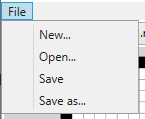
\includegraphics[height=4cm,keepaspectratio]{obr/menu}
		\vspace*{4mm}
		\caption{Hlavní menu}
		\label{obr:menu}
	\end{minipage}%
	\begin{minipage}{.5\textwidth}
		\centering
		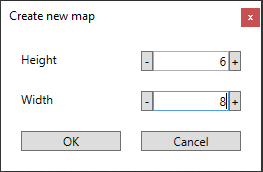
\includegraphics[height=4cm]{obr/newMapDialog}
		\vspace*{4mm}
		\caption{Dialog pro vytvoření nové mapy}
		\label{obr:newMapDialog}
	\end{minipage}
\end{figure}

\subsubsection{2 -- Záložky}
Aplikace umožňuje mít otevřeno několik map zároveň a přepínat mezi nimi pomocí záložek. Všechny funkce aplikace probíhají na aktuálně zvolené mapě.

\subsubsection{3 -- Mapa prostředí}
Prostředí je v aplikaci představováno sítí čtverců, kde bílé čtverce představují přípustné stavy a černé čtverce reprezentují překážky (nepřípustné stavy). Výchozí stavy robotů jsou zobrazeny jako zelené kruhy a cílové stavy jako kruhy červené. Stavy se stejnými čísly přísluší stejnému robotu. Stavy lze přidávat kliknutím levým tlačítkem myši v závislosti na vybraném módu na postranním panelu (4), pravým tlačítkem daný stav smažeme.

\subsubsection{4 -- Postranní panel}
Postranní panel obsahuje dvě záložky:
\begin{itemize}
	\item Editor (obrázek \ref{obr:sideEditor}) -- Obsahuje možnosti týkající se editoru mapy prostředí. Tlačítko \emph{Clear all} smaže z mapy všechny překážky a výchozí a cílové stavy robotů. Tlačítko \emph{Clear robots} smaže pouze výchozí a cílové stavy, překážky ponechá. Přepínačem \emph{Draw} je možné vybrat mód kreslení do mapy. Možnost \emph{Render graph} zobrazí v mapě hrany grafu, který reprezentuje toto prostředí. Toto zobrazení můžeme vidět na obrázku \ref{obr:renderGraph}
	\begin{figure}[htb]
		\begin{center}
			\includegraphics*[height=4cm,keepaspectratio]{obr/sideEditor}
		\end{center}
		\caption{Postranní panel -- záložka Editor}
		\label{obr:sideEditor}
	\end{figure}

\begin{figure}[htb]
\begin{center}
	\includegraphics*[height=10cm,keepaspectratio]{obr/renderGraph}
\end{center}
\caption{Zobrazení grafu v mapě (fialová)}
\label{obr:renderGraph}
\end{figure}
	
	\item Search (obrázek \ref{obr:sideSearch}) -- V této záložce si může uživatel vybrat ve výběrovníku požadovaný algoritmus. Tlačítkem \emph{Run search} se spustí hledání pomocí vybraného algoritmu. Po dokončení hledání se pod tímto tlačítkem zobrazí výsledky s těmito informacemi: počet úspěšně nalezených cest, čas inicializace algoritmu, čas potřebný k hledání a délka nejkratší cesty.
	\begin{figure}[htb]
		\begin{center}
			\includegraphics*[height=4cm,keepaspectratio]{obr/sideSearch}
		\end{center}
		\caption{Postranní panel -- záložka Search}
		\label{obr:sideSearch}
	\end{figure}
\end{itemize}

Po dokončení hledání jsou v mapě zobrazeny nalezené cesty, odlišené barevně pro lepší přehlednost. Příklad můžeme vidět na obrázku~\ref{obr:foundPaths}.

\begin{figure}[htb]
	\begin{center}
		\includegraphics*[height=10cm,keepaspectratio]{obr/foundPaths}
	\end{center}
	\caption{Zobrazení nalezených cest}
	\label{obr:foundPaths}
\end{figure}

\section{Plug-in systém}\label{sec:plugins}
Aplikace podporuje programování plánovacích algoritmů nezávisle na ostatních funkcích programu. Tohoto je dosaženo pomocí vrstvy abstrakce, jejíž schéma můžeme vidět na obrázku \ref{obr:pluginsSchema}. Uživatel ovládá aplikaci pomocí grafického rozhraní, které je obsaženo v projektu \texttt{WPF}. Programová logika je obsažena v projektu \texttt{Core}, která pomocí veřejných rozhraní (angl. interface) a abstraktních tříd provádí plánování cest robotů.

\begin{figure}[htb]
	\begin{center}
		\includegraphics*[width=15cm,keepaspectratio]{obr/pluginsSchema}
	\end{center}
	\caption{Schéma architektury }
	\label{obr:pluginsSchema}
\end{figure}

Uživatel může naprogramovat vlastní algoritmus v jazyce C\texttt{\#}, který aplikace při startu naimportuje a je možné jej použít stejně jako zabudované algoritmy. Pro implementaci algoritmu je nutné vytvořit třídu, která dědí z abstraktní třídy \texttt{AbstractAlgo}, případně rozhraní \texttt{IAlgo}. Vlastnosti a funkce této třídy jsou následující:
\begin{itemize}
	\item \texttt{Graph} -- graf reprezentující danou mapu prostředí
	%\item \texttt{Logger} -- rozhraní umožňující zápis informací o běhu algoritmu
	\item \texttt{Name} -- název algoritmu
	\item \texttt{Robots} -- seznam robotů s danými vlastnostmi (start, cíl, nalezená cesta atd.)
	\item \texttt{Initialize()} -- funkce volaná na začátku hledání
	\item \texttt{RobotFactory(start, target)} -- funkce vytvářející instanci robota, umožňující její rozšíření uživatelem
	\item \texttt{RunSearch()} -- funkce obsahující vlastní implementaci plánovacího algoritmu
\end{itemize}

Sestavenou knihovnu \texttt{.dll} musí uživatel před spuštěním aplikace umístit do složky \texttt{plugins}, ve které se nachází i textový soubor \texttt{readme.md} s bližšími informacemi jak postupovat při implementaci.




\section{MovingAI benchmarks}\label{sec:movingAI}
Aplikace podporuje otevírání a ukládání map ve formátu, který byl zaveden Sturtevantem [Sturtevant] v jeho článku \emph{Benchmarks for Grid-Based Pathfinding}. Jedná se o sadu mřížkových map, která je k dispozici online (https://movingai.com/benchmarks/). Tato sada obsahuje mapy z komerčních počítačových her (např. Baldurs Gate II, Warcraft III a další), mapy z městských prostředí (Berlín, Londýn, ...), mapy bludišť a další náhodně vygenerované mapy. Tyto sady jsou běžně používané ve vědeckých výzkumech pro srovnávání výsledků jednotlivých algoritmů. Příklady těchto map můžeme vidět na obrázku~\ref{obr:mapy}.

% TODO dávkovací režim

\begin{figure}
	\centering
	\begin{subfigure}{.5\textwidth}
		\centering
		\includegraphics[width=6cm]{obr/AR0300SR}
		\vspace*{4mm}
		\caption{Mapa \texttt{AR0300SR} ze hry Baldurs Gate II}
	\end{subfigure}%
	\begin{subfigure}{.5\textwidth}
		\centering
		\includegraphics[width=6cm]{obr/Boston_0_512}
		\vspace*{4mm}
		\caption{Mapa \texttt{Boston\_0\_512}}
	\end{subfigure}
\vspace*{4mm}
	\caption{Příklady map z MovingAI benchmarks [Sturtevant]}
	\label{obr:mapy}
\end{figure}

\section{Implementované algoritmy}


\chapter{Vyhodnocení výsledků}

\clearpage


%
\cleardoublepage
\chapter*{Závěr}

\addcontentsline{toc}{chapter}{Závěr}
\markboth{ZÁVĚR}{ZÁVĚR}

Cílem této práce bylo popsat problematiku plánování cesty více robotů. První část práce se věnovala popisu navigace robota a jejích součástí -- mapování, tj. zpracování a~reprezentaci prostředí, a plánování cesty, tj. konkrétním metodám. Další část se věnovala popisu vybraných algoritmů používaných pro plánování cesty více robotů ve statickém prostředí. Praktická část práce spočívala v implementaci simulačního prostředí, ve kterém byly poté dané algoritmy otestovány ve čtyřech různých prostředích.

K implementaci bylo vybráno 5 algoritmů -- Local Repair A*, vlastní implementace D* Lite pro více robotů nazvaná Multi Agent D* Lite, Cooperative A* a jeho varianty Hierarchical Cooperative A* a Windowed Hierarchical A*.

Navržené simulační prostředí aplikace umožňuje vytváření, ukládání a načítání map vlastních, případně map ze sady benchmarků MovingAI. Navíc aplikace podporuje jednoduchou implementaci dalších algoritmů pomocí plug-in systému, kdy není potřeba zasahovat do aplikační logiky aplikace. Tohoto lze využít např. ve výuce nebo dalším výzkumu na toto téma.

Algoritmy byly srovnány ve čtyřech experimentech, které se lišily jak velikostí, tak i~topologií mapy. V každém experimentu byl postupně navyšován počet robotů od 1 do 60 a porovnávány následující informace: úspěšnost nalezení cesty všemi roboty, čas běhu algoritmu, průměrný počet expandovaných uzlů na jednoho robota a~průměrná odchylka od optimální délky nalezené cesty.

Algoritmus Local Repair A* je jednoduchý na implementaci, avšak při vyšším počtu robotů dochází k častému přeplánování, tudíž k navýšení počtu expandovaných uzlů a~času potřebného pro běh algoritmu. Navíc dochází k selhání nalezení cest pro všechny roboty. Algoritmus Multi Agent D* Lite byl navržen pro snížení počtu expandovaných uzlů při přeplánování. V tomto je algoritmus úspěšný, ve všech experimentech dosáhl nejmenšího počtu expandovaných uzlů ze všech algoritmů. Stejně jako u Local Repair A* však může dojít k selhání nalezení cesty pro všechny roboty. Navíc jeho základem je nalezení hrany grafu takové, která minimalizuje danou funkci, která je ovšem v této implementaci problematická, tudíž algoritmus nedosahuje takových časů jako ostatní algoritmy. V budoucnosti by se tento problém mohl vyřešit lepší implementací nalezení dané hrany, případně např. paralelizací výpočtu. Cooperative A* se ukázal jako nepraktický, protože expanduje velký počet zbytečných uzlů, což při složitých velkých mapách vede k~obrovskému nárůstu výpočetního času. Hierarchical Cooperative A* řeší tento problém výpočtem odhadu vzdáleností v abstraktním prostoru pomocí Reverse Resumable A* algoritmu. Windowed Hierarchical Cooperative A* dále rozšiřuje abstrakci o zavedení tzv. okna, ve kterém uvažuje ostatní roboty a dále už ne. Oba tyto algoritmy obstály ve všech experimentech, kdy časová náročnost i odchylky od optimální délky cesty byly nejmenší ze všech algoritmů, avšak za cenu většího počtu expandovaných uzlů.



% nutné
\phantomsection
\addcontentsline{toc}{chapter}{Literatura}
\begin{thebibliography}{99}

\bibitem{Meyer2003}
MEYER, Jean-Arcady a David FILLIAT. Map-based navigation in mobile robots. In: \textit{Cognitive Systems Research} [online]. 2003, s.~283-317 [cit. 2020-06-18]. DOI: 10.1016/S1389-0417(03)00007-X. ISSN 13890417. Dostupné z: https://linkinghub.elsevier.com/retrieve/pii/S138904170300007X

\bibitem{Stachniss2009}
STACHNISS, Cyrill. \textit{Robotic Mapping and Exploration} [online]. Berlin: Heidelberg: Springer Berlin Heidelberg, 2009 [cit. 2020-06-21]. DOI: 10.1007/978-3-642-01097-2. ISBN 978-3-642-01096-5. Dostupné z: https://www.researchgate.net/publication/220688303

\bibitem{Koubaa20180406}
KOUBAA, Anis, Hachemi BENNACEUR, Imen CHAARI, et al. Introduction to Mobile Robot Path Planning. In: \textit{Robot Path Planning and Cooperation} [online]. Cham: Springer International Publishing, 2018, 2018-04-06, s.~3-12 [cit. 2020-06-21]. Studies in Computational Intelligence. DOI: 10.1007/978-3-319-77042-0\_1. ISBN 978-3-319-77040-6. Dostupné z: http://link.springer.com/10.1007/978-3-319-77042-0\_1

\bibitem{LaValle2006}
LAVALLE, Steven Michael. \textit{Planning algorithms} [online]. New York: Cambridge University Press, 2006 [cit. 2020-06-21]. ISBN 9780521862059. Dostupné z: http://lavalle.pl/planning/

\bibitem{Parker2009}
PARKER, Lynne E. Multiple Mobile Robot Teams, Path Planning and Motion Coordination in. In: \textit{Encyclopedia of Complexity and Systems Science} [online]. New York, NY: Springer New York, 2009, 2009, s.~5783-5800 [cit. 2020-06-18]. DOI: 10.1007/978-0-387-30440-3\_344. ISBN 978-0-387-75888-6. Dostupné z: http://link.springer.com/10.1007/978-0-387-30440-3\_344

\bibitem{Ferguson2005}
FERGUSON, Dave, Maxim LIKHACHEV a Anthony STENTZ. A Guide to Heuristic-based Path Planning. In: \textit{Proceedings of the international workshop on planning under uncertainty for autonomous systems, international conference on automated planning and scheduling (ICAPS)} [online]. 2005, s.~9-18 [cit. 2020-06-21]. Dostupné z: https://www.cs.cmu.edu/afs/cs.cmu.edu/Web/People/maxim/files/hsplanguide\_icaps05ws.pdf

\bibitem{Yu20140122}
YU, Wentao, Jun PENG, Xiaoyong ZHANG a Kuo-Chi LIN. A Cooperative Path Planning Algorithm for a Multiple Mobile Robot System in a Dynamic Environment. In: \textit{International Journal of Advanced Robotic Systems} [online]. 2014 [cit. 2020-06-21]. DOI: 10.5772/58832. ISSN 1729-8814. Dostupné z: http://journals.sagepub.com/doi/10.5772/58832

\bibitem{Dudek1996}
DUDEK, Gregory, Michael R.M. JENKIN, Evangelos MILIOS a David WILKES. A taxonomy for multi-agent robotics. In: \textit{Autonomous Robots} [online]. 1996 [cit. 2020-06-21]. DOI: 10.1007/BF00240651. ISSN 0929-5593. Dostupné z: http://link.springer.com/10.1007/BF00240651

\bibitem{Yan20130104}
YAN, Zhi, Nicolas JOUANDEAU a Arab Ali CHERIF. A Survey and Analysis of Multi-Robot Coordination. In: \textit{International Journal of Advanced Robotic Systems} [online]. 2013 [cit. 2020-06-21]. DOI: 10.5772/57313. ISSN 1729-8814. Dostupné z: http://journals.sagepub.com/doi/10.5772/57313

\bibitem{Asma2017}
ASMA, Ayari a Bouamama SADOK. Dynamic Distributed PSO joints elites in Multiple Robot Path Planning Systems: theoretical and practical review of new ideas. In: \textit{Procedia Computer Science} [online]. 2017, s.~1082-1091 [cit. 2020-06-21]. DOI: 10.1016/j.procs.2017.08.128. ISSN 18770509. Dostupné z: https://linkinghub.elsevier.com/retrieve/pii/S1877050917314850

\bibitem{Solovey20160408}
SOLOVEY, Kiril, Oren SALZMAN a Dan HALPERIN. Finding a needle in an exponential haystack: Discrete RRT for exploration of implicit roadmaps in multi-robot motion planning. In: \textit{The International Journal of Robotics Research} [online]. 2016, s.~501-513 [cit. 2020-06-21]. DOI: 10.1177/0278364915615688. ISSN 0278-3649. Dostupné z: http://journals.sagepub.com/doi/10.1177/0278364915615688

\bibitem{Silver2005}
SILVER, David. Cooperative Pathfinding. In: \textit{Proceedings of the First AAAI Conference on Artificial Intelligence and Interactive Digital Entertainment} [online]. 2005, s.~117-122 [cit. 2020-06-21]. Dostupné z: https://www.aaai.org/Papers/AIIDE/2005/AIIDE05-020.pdf

\bibitem{Alajlan2013}
ALAJLAN, Maram, Anis KOUBAA, Imen CHAARI, Hachemi BENNACEUR a Adel AMMAR. Global path planning for mobile robots in large-scale grid environments using genetic algorithms. In: \textit{2013 International Conference on Individual and Collective Behaviors in Robotics (ICBR)} [online]. IEEE, 2013, 2013, s.~1-8 [cit. 2020-06-21]. DOI: 10.1109/ICBR.2013.6729271. ISBN 978-1-4799-2813-2. Dostupné z: http://ieeexplore.ieee.org/document/6729271/

\bibitem{Hart1968}
HART, Peter, Nils NILSSON a Bertram RAPHAEL. A Formal Basis for the Heuristic Determination of Minimum Cost Paths. In: \textit{IEEE Transactions on Systems Science and Cybernetics} [online]. 1968, s.~100-107 [cit. 2020-06-21]. DOI: 10.1109/TSSC.1968.300136. ISSN 0536-1567. Dostupné z: http://ieeexplore.ieee.org/document/4082128/

\bibitem{Silver2006}
SILVER, David. Cooperative Pathfinding. In: \textit{AI Game Programming Wisdom 3} [online]. Charles River Media, 2006, s.~99-111 [cit. 2020-06-21]. ISBN 9781584504573. Dostupné z: https://www.davidsilver.uk/wp-content/uploads/2020/03/coop-path-AIWisdom-1.pdf

\bibitem{Koenig2004}
KOENIG, Sven, Maxim LIKHACHEV a David FURCY. Lifelong Planning A. In: \textit{Artificial Intelligence} [online]. 2004, s.~93-146 [cit. 2020-06-22]. DOI: 10.1016/j.artint.2003.12.001. ISSN 00043702. Dostupné z: https://linkinghub.elsevier.com/retrieve/pii/S000437020300225X

\bibitem{Stentz1997}
STENTZ, Anthony. Optimal and Efficient Path Planning for Partially Known Environments. In: \textit{Intelligent Unmanned Ground Vehicles} [online]. Boston, MA: Springer US, 1997, 1997, s.~203-220 [cit. 2020-06-22]. DOI: 10.1007/978-1-4615-6325-9\_11. ISBN 978-1-4613-7904-1. Dostupné z: http://link.springer.com/10.1007/978-1-4615-6325-9\_11

\bibitem{Stentz1995}
STENTZ, Anthony. The Focussed D* algorithm for real-time replanning. In: \textit{Proceedings of the 14th international joint conference on Artificial intelligence - Volume 2} [online]. San Francisco: Morgan Kaufmann Publishers, 1995, s.~1662-1669 [cit. 2020-06-22]. Dostupné z: https://www.ijcai.org/Proceedings/95-2/Papers/082.pdf

\bibitem{Koenig2002}
KOENIG, Sven a Maxim LIKHACHEV. D* Lite. In: \textit{Eighteenth national conference on Artificial intelligence} [online]. American Association for Artificial Intelligence, 2002, s.~476-483 [cit. 2020-06-22]. Dostupné z: https://www.aaai.org/Papers/AAAI/2002/AAAI02-072.pdf


\bibitem{ECMA}
\textit{ECMA-334: C\# Language Specification} [online]. Geneva: ECMA International, 2017 [cit. 2020-06-21]. Dostupné z: https://www.ecma-international.org/publications/standards/Ecma-334.htm

\bibitem{MSDOCS}
\textit{Microsoft Docs: Technical documentation, API, and code examples} [online]. Microsoft, c2020 [cit. 2020-06-21]. Dostupné z: https://docs.microsoft.com/en-us/

\bibitem{Stylet}
Stylet. \textit{GitHub} [online]. c2020 [cit. 2020-06-21]. Dostupné z: https://github.com/canton7/Stylet

\bibitem{QuickGraph}
QuickGraph. \textit{GitHub} [online]. c2020 [cit. 2020-06-21]. Dostupné z: https://github.com/YaccConstructor/QuickGraph

\bibitem{HSPQ}
High Speed Priority Queue. \textit{GitHub} [online]. c2020 [cit. 2020-06-21]. Dostupné z: https://github.com/BlueRaja/High-Speed-Priority-Queue-for-C-Sharp

\bibitem{Sturtevant2012}
STURTEVANT, N. R. Benchmarks for Grid-Based Pathfinding. In: \textit{IEEE Transactions on Computational Intelligence and AI in Games} [online]. 2012, s.~144-148 [cit. 2020-05-13]. DOI: 10.1109/TCIAIG.2012.2197681. ISSN 1943-068X. Dostupné z: http://ieeexplore.ieee.org/document/6194296/

\bibitem{Alajlan2013}
ALAJLAN, Maram, Anis KOUBAA, Imen CHAARI, Hachemi BENNACEUR a Adel AMMAR. Global path planning for mobile robots in large-scale grid environments using genetic algorithms. In: \textit{2013 International Conference on Individual and Collective Behaviors in Robotics (ICBR)} [online]. IEEE, 2013, 2013, s.~1-8 [cit. 2020-06-23]. DOI: 10.1109/ICBR.2013.6729271. ISBN 978-1-4799-2813-2. Dostupné z: http://ieeexplore.ieee.org/document/6729271/
\bibitem{Gao2008}
GAO, Meijuan, Jin XU, Jingwen TIAN a Hao WU. Path Planning for Mobile Robot Based on Chaos Genetic Algorithm. In: \textit{2008 Fourth International Conference on Natural Computation} [online]. IEEE, 2008, 2008, s.~409-413 [cit. 2020-06-23]. DOI: 10.1109/ICNC.2008.627. ISBN 978-0-7695-3304-9. Dostupné z: http://ieeexplore.ieee.org/document/4667315/
\bibitem{Lamini2018}
LAMINI, Chaymaa, Said BENHLIMA a Ali ELBEKRI. Genetic Algorithm Based Approach for Autonomous Mobile Robot Path Planning. In: \textit{Procedia Computer Science} [online]. 2018, s.~180-189 [cit. 2020-06-23]. DOI: 10.1016/j.procs.2018.01.113. ISSN 18770509. Dostupné z: https://linkinghub.elsevier.com/retrieve/pii/S187705091830125X
\bibitem{Liang2015}
LIANG, Jun-Hao a Ching-Hung LEE. Efficient collision-free path-planning of multiple mobile robots system using efficient artificial bee colony algorithm. In: \textit{Advances in Engineering Software} [online]. 2015, s.~47-56 [cit. 2020-06-23]. DOI: 10.1016/j.advengsoft.2014.09.006. ISSN 09659978. Dostupné z: https://linkinghub.elsevier.com/retrieve/pii/S0965997814001495
\bibitem{Karaboga2005}
KARABOGA, Dervis. \textit{An idea based on honey bee swarm for numerical optimization} [online]. 2005 [cit. 2020-06-23]. Dostupné z: https://www.semanticscholar.org/paper/AN-IDEA-BASED-ON-HONEY-BEE-SWARM-FOR-NUMERICAL-Karaboga/cf20e34a1402a115523910d2a4243929f6704db1
\bibitem{Dreo2006}
DRÉO, Johann. Aco TSP. In: \textit{Wikipedia: the free encyclopedia} [online]. San Francisco (CA): Wikimedia Foundation, 2020, 2006 [cit. 2020-06-22]. Dostupné z: https://en.wikipedia.org/wiki/File:Aco\_TSP.svg
\bibitem{Nakisa20140901}
NAKISA. A SURVEY: PARTICLE SWARM OPTIMIZATION BASED ALGORITHMS TO SOLVE PREMATURE CONVERGENCE PROBLEM. In: \textit{Journal of Computer Science} [online]. 2014, s.~1758-1765 [cit. 2020-06-22]. DOI: 10.3844/jcssp.2014.1758.1765. ISSN 1549-3636. Dostupné z: http://thescipub.com/abstract/10.3844/jcssp.2014.1758.1765
\bibitem{Asma2017}
ASMA, Ayari a Bouamama SADOK. Dynamic Distributed PSO joints elites in Multiple Robot Path Planning Systems: theoretical and practical review of new ideas. In: \textit{Procedia Computer Science} [online]. 2017, s.~1082-1091 [cit. 2020-06-22]. DOI: 10.1016/j.procs.2017.08.128. ISSN 18770509. Dostupné z: https://linkinghub.elsevier.com/retrieve/pii/S1877050917314850
\bibitem{Kennedy1995}
KENNEDY, J. a R. EBERHART. Particle swarm optimization. In: \textit{Proceedings of ICNN'95 - International Conference on Neural Networks} [online]. IEEE, 1995, s.~1942-1948 [cit. 2020-06-22]. DOI: 10.1109/ICNN.1995.488968. ISBN 0-7803-2768-3. Dostupné z: http://ieeexplore.ieee.org/document/488968/
\bibitem{SinghPal20131218}
SINGHPAL, Narendra a Sanjeev SHARMA. Robot Path Planning using Swarm Intelligence: A Survey. In: \textit{International Journal of Computer Applications} [online]. 2013, s.~5-12 [cit. 2020-06-22]. DOI: 10.5120/14498-2274. ISSN 09758887. Dostupné z: http://research.ijcaonline.org/volume83/number12/pxc3892274.pdf
\bibitem{Masehian2004}
MASEHIAN, Ellips a M. R. AMIN-NASERI. A voronoi diagram-visibility graph-potential field compound algorithm for robot path planning. In: \textit{Journal of Robotic Systems} [online]. 2004, s.~275-300 [cit. 2020-06-22]. DOI: 10.1002/rob.20014. ISSN 0741-2223. Dostupné z: http://doi.wiley.com/10.1002/rob.20014
\bibitem{Wallar2014}
WALLAR, Alex a Erion PLAKU. Path planning for swarms in dynamic environments by combining probabilistic roadmaps and potential fields. In: \textit{2014 IEEE Symposium on Swarm Intelligence} [online]. IEEE, 2014, 2014, s.~1-8 [cit. 2020-06-22]. DOI: 10.1109/SIS.2014.7011808. ISBN 978-1-4799-4458-3. Dostupné z: http://ieeexplore.ieee.org/document/7011808/
\bibitem{Abd Algfoor2015}
ABD ALGFOOR, Zeyad, Mohd Shahrizal SUNAR a Hoshang KOLIVAND. A Comprehensive Study on Pathfinding Techniques for Robotics and Video Games. In: \textit{International Journal of Computer Games Technology} [online]. 2015, s.~1-11 [cit. 2020-06-22]. DOI: 10.1155/2015/736138. ISSN 1687-7047. Dostupné z: http://www.hindawi.com/journals/ijcgt/2015/736138/
\bibitem{Tsourdos2010}
TSOURDOS, Antonios, Brian WHITE a Madhavan SHANMUGAVEL. \textit{Cooperative Path Planning of Unmanned Aerial Vehicles} [online]. Washington, DC: American Institute of Aeronautics and Astronautics, 2010 [cit. 2020-06-22]. DOI: 10.2514/4.867798. ISBN 978-1-60086-779-8.
\bibitem{Opfer20111202}
OPFER, Stephan, Hendrik SKUBCH a Kurt GEIHS. Cooperative Path Planning for Multi-Robot Systems in Dynamic Domains. In: \textit{Mobile Robots - Control Architectures, Bio-Interfacing, Navigation, Multi Robot Motion Planning and Operator Training} [online]. InTech, 2011, 2011-12-02 [cit. 2020-06-22]. DOI: 10.5772/26440. ISBN 978-953-307-842-7. Dostupné z: http://www.intechopen.com/books/mobile-robots-control-architectures-bio-interfacing-navigation-multi-robot-motion-planning-and-operator-training/cooperative-path-planning-for-multi-robot-systems-in-dynamic-domains
\bibitem{Masehian2007}
MASEHIAN, Ellips a Davoud SEDIGHIZADEH. Classic and Heuristic Approaches in Robot Motion Planning: A Chronological Review. In: \textit{International Journal of Mechanical, Industrial Science and Engineering} [online]. World Academy of Science, Engineering and Technology, 2007 [cit. 2020-06-22]. DOI: 10.5281/zenodo.1074972. Dostupné z: https://www.researchgate.net/publication/249714449
\bibitem{Liu2006}
LIU, Shirong, Linbo MAO a Jinshou YU. Path Planning Based on Ant Colony Algorithm and Distributed Local Navigation for Multi-Robot Systems. In: \textit{2006 International Conference on Mechatronics and Automation} [online]. IEEE, 2006, 2006, s.~1733-1738 [cit. 2020-06-23]. DOI: 10.1109/ICMA.2006.257476. ISBN 1-4244-0465-7. Dostupné z: http://ieeexplore.ieee.org/document/4026354/
	
\bibitem{Patel19972020}
PATEL, Amit. Heuristics. \textit{Amit-s A* Pages} [online]. 2020 [cit. 2020-06-23]. Dostupné z: https://theory.stanford.edu/~amitp/GameProgramming/Heuristics.html
\bibitem{Goldenberg2012}
GOLDENBERG, Meir, Ariel FELNER, Roni STERN, Guni SHARON a Jonathan SCHAEFFER. A* variants for optimal multi-agent pathfinding. In: \textit{Workshops at the Twenty-Sixth AAAI Conference on Artificial Intelligence} [online]. 2012, s.~19-25 [cit. 2020-06-23]. Dostupné z: https://www.aaai.org/ocs/index.php/WS/AAAIW12/paper/viewPaper/5233
\bibitem{STANDLEY}
STANDLEY, Trevor Scott. Finding optimal solutions to cooperative pathfinding problems. In: \textit{Twenty-Fourth AAAI Conference on Artificial Intelligence} [online]. 2010, s.~173-178 [cit. 2020-06-23]. Dostupné z: https://www.aaai.org/ocs/index.php/AAAI/AAAI10/paper/view/1926
\bibitem{Kraft2017}
KRAFT, Aaron R. Abstraction Hierarchies for Multi-Agent Pathfinding. In: \textit{Electronic Theses and Dissertations.~1247.} [online]. University of Denver, 2017, 73 p. [cit. 2020-06-23]. Dostupné z: https://digitalcommons.du.edu/etd/1247

\bibitem{Dijkstra1959}
DIJKSTRA, E. W. A note on two problems in connexion with graphs. In: \textit{Numerische Mathematik} [online]. 1959, s.~269-271 [cit. 2020-06-23]. DOI: 10.1007/BF01386390. ISSN 0029-599X. Dostupné z: http://link.springer.com/10.1007/BF01386390
	
	
\end{thebibliography}% nutné

\chapter*{Seznam použitých zkratek a symbolů}
\symbolsize=3.5cm% sirka sloupecku pro symboly, je mozno zmensit pokud jsou kratke
\addcontentsline{toc}{chapter}{Seznam použitých zkratek a symbolů}
\markboth{SEZNAM POUŽITÝCH ZKRATEK A SYMBOLŮ}{SEZNAM POUŽITÝCH ZKRATEK A SYMBOLŮ}
\begin{symboly}
	\item[$\Phi$] popis symbolu


\end{symboly}
% nutné
\chapter*{Seznam příloh}
\addcontentsline{toc}{chapter}{Seznam příloh}
\markboth{SEZNAM PŘÍLOH}{SEZNAM PŘÍLOH}
%Součástí práce je CD, které obsahuje:
\begin{itemize}
	\item \verb|NURBS.exe| -- spustitelný soubor programu pro vytváření rotačních NURBS ploch
\end{itemize}
% není povinné
\end{document}
